\documentclass{article}
\usepackage[utf8x]{inputenc}
\usepackage{ucs}
\usepackage{amsmath} 
\usepackage{amsfonts}
\usepackage{upgreek}
\usepackage[english,russian]{babel}
\usepackage{graphicx}
\usepackage{float}
\usepackage{textcomp}
\usepackage{hyperref}
\usepackage{geometry}
  \geometry{left=2cm}
  \geometry{right=1.5cm}
  \geometry{top=1cm}
  \geometry{bottom=2cm}
\usepackage{tikz}
\usepackage{ccaption}
\usepackage{multicol}


\usepackage{listings}


\begin{document}
\pagestyle{plain}
\lstset{
  language=C,                % choose the language of the code
  basicstyle=\linespread{1.1}\ttfamily,
  columns=fixed,
  fontadjust=true,
  basewidth=0.5em,
  keywordstyle=\color{blue}\bfseries,
  commentstyle=\color{gray},
  stringstyle=\ttfamily\color{orange!50!black},
  showstringspaces=false,
  numbersep=5pt,
  numberstyle=\tiny\color{black},
  numberfirstline=true,
  stepnumber=1,                   % the step between two line-numbers.        
  numbersep=10pt,                  % how far the line-numbers are from the code
  backgroundcolor=\color{white},  % choose the background color. You must add \usepackage{color}
  showstringspaces=false,         % underline spaces within strings
  captionpos=b,                   % sets the caption-position to bottom
  breaklines=true,                % sets automatic line breaking
  breakatwhitespace=true,         % sets if automatic breaks should only happen at whitespace
  xleftmargin=.2in,
  extendedchars=\true,
  keepspaces = true,
}
\lstset{literate=%
   *{0}{{{\color{red!20!violet}0}}}1
    {1}{{{\color{red!20!violet}1}}}1
    {2}{{{\color{red!20!violet}2}}}1
    {3}{{{\color{red!20!violet}3}}}1
    {4}{{{\color{red!20!violet}4}}}1
    {5}{{{\color{red!20!violet}5}}}1
    {6}{{{\color{red!20!violet}6}}}1
    {7}{{{\color{red!20!violet}7}}}1
    {8}{{{\color{red!20!violet}8}}}1
    {9}{{{\color{red!20!violet}9}}}1
}
\renewcommand{\thesubsection}{\arabic{subsection}}
\makeatletter
\def\@seccntformat#1{\@ifundefined{#1@cntformat}%
   {\csname the#1\endcsname\quad}%    default
   {\csname #1@cntformat\endcsname}}% enable individual control
\newcommand\section@cntformat{}     % section level 
\newcommand\subsection@cntformat{Задача \thesubsection.\space} % subsection level
\newcommand\subsubsection@cntformat{\thesubsubsection.\space} % subsubsection level
\makeatother


\title{Семинар \#6: Структуры. Домашнее задание.\vspace{-5ex}}\date{}\maketitle

\subsection{Треугольник}
Для описания треугольников на плоскости были определены структуры \texttt{Point} и \texttt{Triangle}:
\begin{lstlisting}
struct point 
{
    double x, y;
};
typedef struct point Point;

struct triangle 
{
    Point a, b, c;
};
typedef struct triangle Triangle;
\end{lstlisting}
Напишите следующие функции для работы с этими структурами:
\begin{itemize}
\item Функцию \texttt{print\_point}, которая будет принимать точку и печатать её в формате \texttt{(1.23, 4.56)}. То есть в круглых скобках, через запятую и с двумя знаками после запятой.

\item Функцию \texttt{print\_triangle}, которая будет принимать на вход треугольник и печатать координаты треугольника в следующем формате: \texttt{\{(1.00, 0.00), (0.50, 2.00), (0.00, 1.50)\}}.

\item Функцию \texttt{distance}, которая будет принимать на вход 2 точки и возвращать расстояние между ними.

\item Функцию \texttt{get\_triangle\_perimeter}, которая будет принимать треугольник по константному указателю и возвращать его периметр.

\item Функцию \texttt{get\_triangle\_area}, которая будет принимать на вход треугольник по константному указателю и возвращать его площадь. Можно использовать формулу Герона.

\item Функцию \texttt{moved\_triangle}, которая будет принимать на вход треугольник по константному указателю и одну точку (она будет играть роль вектора-перемещения). Функция должна возвращать новый треугольник, у которого все координаты будут передвинуты на вектор-перемещение.

\item Функцию \texttt{move\_triangle}, которая будет принимать на вход треугольник по указателю и одну точку (она будет играть роль вектора-перемещения). Функция должна менять передаваемый ей треугольник.
\end{itemize}

\subsection{Рецензии на компьютерные игры}
На вход программе приходит информация о рецензиях компьютерных игр. В первой строке содержится число \texttt{n} - количество игр. Далее идут \texttt{n} строк. В каждой строке содержится название игры, заканчивающееся двоеточием сразу после идёт целое число \texttt{k} -- количество оценок, которые эта игра получила, затем идут \texttt{k} оценок. Оценка, это число от 1 до 10. Нужно отсортировать все игры по средней оценке и напечатать название игр и их среднюю оценку.

\begin{center}
\begin{tabular}{ l | l }
 вход & выход \\ \hline
 \texttt{5} & 								  \texttt{The Cube, 8.286} \\
 \texttt{Need For Speed: 6 6 1 2 7 5 4} &      \texttt{Metal Power, 5.900 } \\
 \texttt{Sector: 3 1 4 2} & 					  \texttt{Principle Of Chaos 2, 5.200} \\
 \texttt{The Cube: 7 9 8 7 9 8 10 7} &          \texttt{Need For Speed, 4.667 } \\
 \texttt{Principle Of Chaos 2: 5 4 3 6 5 7} &     \texttt{Sector, 2.333} \\
 \texttt{Metal Power: 10 8 5 3 9 6 2 6 7 5 8} & \\
\end{tabular}
\end{center}
Протестировать программу можно на файле \texttt{videogames.txt}.


\newpage

\subsection{Создание указателей}
Решения всех подзадач этой части -- одна строка. Результат выполнения задания -- \texttt{.txt} файл, который содержит все эти строки.
\begin{enumerate}
\item В следующей программе создаётся переменная \texttt{a} типа \texttt{int}:
\begin{lstlisting}
int main() 
{
    int a = 1234;
    // Тут нужно написать 1 строку кода
}
\end{lstlisting}
Создайте указатель \texttt{p} и инициализируйте его адресом переменной \texttt{a}.


\item В следующей программе создаётся переменная \texttt{a} типа \texttt{double}:
\begin{lstlisting}
int main() 
{
    double a = 12.34;
    // Тут нужно написать 1 строку кода
}
\end{lstlisting}
Создайте указатель \texttt{p} и инициализируйте его адресом переменной \texttt{a}.

\item В следующей программе создаётся переменная \texttt{a} типа \texttt{char}:
\begin{lstlisting}
int main() 
{
    char a = ')';
    // Тут нужно написать 1 строку кода
}
\end{lstlisting}
Создайте указатель \texttt{p} и инициализируйте его адресом переменной \texttt{a}.

\item В следующей программе создаётся массив \texttt{array} из элементов типа \texttt{int}:
\begin{lstlisting}
int main() 
{
    int array[5] = {10, 20, 30, 40, 50};
    // Тут нужно написать 1 строку кода
}
\end{lstlisting}
Создайте указатель \texttt{p} и сделайте так, чтобы он указывал на первый элемент массива (индекс \texttt{0}).


\item В следующей программе создаётся строка -- массив \texttt{str} из элементов типа \texttt{char}:
\begin{lstlisting}
int main() 
{
    char str[20] = "Sapere Aude";
    // Тут нужно написать 1 строку кода
}
\end{lstlisting}
Создайте указатель \texttt{p} и сделайте так, чтобы он указывал на символ \texttt{'A'}  из строки \texttt{str}.

\newpage
\item В следующей программе создаётся структура \texttt{Book} из семинара про структуры:
\begin{lstlisting}
struct book 
{
    char title[50];
    int pages;
    float price;
};
typedef struct book Book;

int main() 
{
    Book b = {"Fahrenheit 451", 400, 700.0};

}
\end{lstlisting}

\begin{enumerate}
\item Создайте указатель \texttt{pb} и сделайте так, чтобы он указывал на структуру \texttt{b}.
\item Создайте указатель \texttt{pprice} и сделайте так, чтобы он указывал на поле \texttt{price} структуры \texttt{b}.
\item Создайте указатель \texttt{pc} и сделайте так, чтобы он указывал символ \texttt{'t'} поля \texttt{title} структуры \texttt{b}.
\end{enumerate} 


\item В следующей программе создаётся переменная \texttt{a} типа \texttt{float} и \texttt{p} указатель, который хранит её адрес:
\begin{lstlisting}
int main() 
{
    float a = 1.2;
    float* p = &a;
    // Тут нужно написать 1 строку кода
}
\end{lstlisting}
Создайте указатель \texttt{pp} и сделайте так, чтобы он указывал на указатель \texttt{p}.


\item В следующей программе создаётся структура \texttt{Book} из семинара про структуры и указатель на неё:
\begin{lstlisting}
struct book 
{
    char title[50];
    int pages;
    float price;
};
typedef struct book Book;

int main() 
{
    Book b = {"Fahrenheit 451", 400, 700.0};
    Book* pb = &b;
    // Тут нужно написать 1 строку кода
}
\end{lstlisting}
Создайте указатель \texttt{ppb} и сделайте так, чтобы он указывал на указатель \texttt{pb}.


\end{enumerate}

\newpage
\subsection{Использование указателей}
Решения всех подзадач этой части -- одна строка. Результат выполнения задания -- \texttt{.txt} файл, который содержит все эти строки.
\begin{enumerate}
\item В следующей программе была создана переменная \texttt{a} и указатель на неё \texttt{p}. Удвойте значение переменной \texttt{a}, используя только указатель \texttt{p}. Нужно использовать указатель \texttt{p}, саму переменную \texttt{a} использовать нельзя.
\begin{multicols}{2}
\begin{lstlisting}
#include <stdio.h>
int main() 
{
    int a = 1234;
    int* p = &a;
    // Тут нужно написать 1 строку кода
    
    printf("%i\n", a);
}
\end{lstlisting}

\vfill \null    
\columnbreak
\vfill \null 

\begin{center}
\vspace{1cm} 
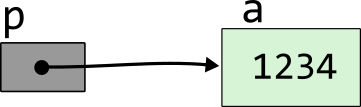
\includegraphics[scale=1]{../images/pointer_schemes/pointer_to_int.png}
\end{center}
\end{multicols}

\item В следующей программе была создана переменная \texttt{a} типа \texttt{float} и указатель на неё \texttt{p}. Возведите значение переменной \texttt{a} в квадрат, используя только указатель \texttt{p}. Нужно использовать только указатель \texttt{p}, саму переменную \texttt{a} использовать нельзя.
\begin{multicols}{2}
\begin{lstlisting}
#include <stdio.h>
int main() 
{
    float a = 1.5;
    float* p = &a;
    // Тут нужно написать 1 строку кода
    
    printf("%f\n", a);
}
\end{lstlisting}

\vfill \null    
\columnbreak
\vfill \null 

\begin{center}
\vspace{1cm} 
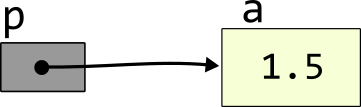
\includegraphics[scale=1]{../images/pointer_schemes/pointer_to_float.png}
\end{center}
\end{multicols}


\item В следующей программе была создана переменная \texttt{a} типа \texttt{char} и указатель на неё \texttt{p}. Переведите символ, хранящийся в переменной \texttt{a} в верхний регистр, используя только указатель \texttt{p}. Нужно использовать только указатель \texttt{p}, саму переменную \texttt{a} использовать нельзя.
\begin{multicols}{2}
\begin{lstlisting}
#include <stdio.h>
int main() 
{
    char a = 't';
    char* p = &a;
    // Тут нужно написать 1 строку кода
    
    printf("%c\n", a);
}
\end{lstlisting}

\vfill \null    
\columnbreak
\vfill \null 

\begin{center}
\vspace{1cm} 
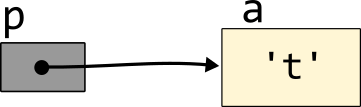
\includegraphics[scale=1]{../images/pointer_schemes/pointer_to_char.png}
\end{center}
\end{multicols}


\newpage
\item В следующей программе был создан массив \texttt{array} переменных  типа \texttt{int} и указатель \texttt{p} на первый элемент массива. 
\begin{multicols}{2}
\begin{lstlisting}
#include <stdio.h>
int main() 
{
    int array[5] = {10, 20, 30, 40, 50};
    int* p = &array[0];

    for (int i = 0; i < 5; ++i) 
        printf("%i ", array[i]);
}
\end{lstlisting}
\vfill \null    
\columnbreak
\vfill \null 
\begin{center}
\vspace{1cm} 
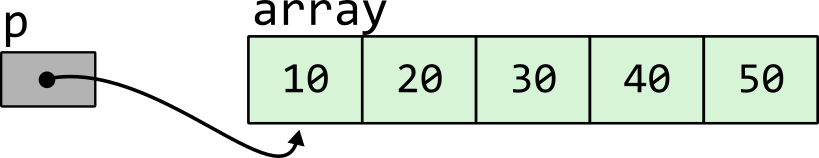
\includegraphics[scale=0.8]{../images/pointer_schemes/pointer_to_int_array.png}
\end{center}
\end{multicols}

\begin{enumerate}
\item Добавьте \texttt{1} к первому элементу массива (\texttt{array[0]}), используя только указатель \texttt{p}. Нужно использовать только указатель \texttt{p}, сам массив \texttt{array} использовать нельзя. Решение -- 1 строка.
\item Добавьте \texttt{1} к четвёртому элементу массива (\texttt{array[3]}), используя только указатель \texttt{p}. Нужно использовать только указатель \texttt{p}, сам массив \texttt{array} использовать нельзя. Менять \texttt{p} тоже нельзя. Решение -- 1 строка.

\item Добавьте \texttt{1} ко всем элементам массива. Нужно использовать только указатель \texttt{p}, сам массив \texttt{array} использовать нельзя. Решение -- 1 цикл.
\end{enumerate}


\item В следующей программе был создан массив \texttt{array} переменных  типа \texttt{int} и указатель \texttt{p} на четвёртый элемент массива (\texttt{array[3]}). 
\begin{multicols}{2}
\begin{lstlisting}
#include <stdio.h>
int main() 
{
    int array[5] = {10, 20, 30, 40, 50};
    int* p = &array[3];
    
    for (int i = 0; i < 5; ++i)
        printf("%i ", array[i]);
}
\end{lstlisting}
\vfill \null    
\columnbreak
\vfill \null 
\begin{center}
\vspace{1cm} 
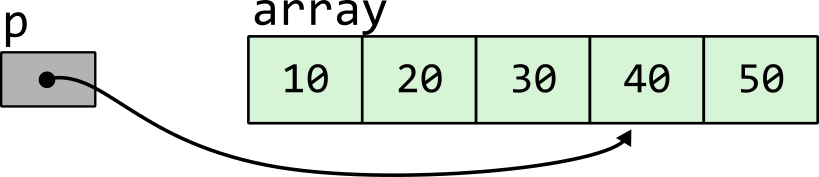
\includegraphics[scale=0.8]{../images/pointer_schemes/pointer_to_int_array_index4.png}
\end{center}
\end{multicols}

\begin{enumerate}
\item Добавьте \texttt{1} к первому элементу массива (\texttt{array[0]}), используя только указатель \texttt{p}. Нужно использовать только указатель \texttt{p}, сам массив \texttt{array} использовать нельзя. Менять \texttt{p} тоже нельзя. Решение -- 1 строка.
\item Добавьте \texttt{1} к пятому элементу массива (\texttt{array[4]}), используя только указатель \texttt{p}. Нужно использовать только указатель \texttt{p}, сам массив \texttt{array} использовать нельзя. Менять \texttt{p} тоже нельзя. Решение -- 1 строка.
\item Добавьте \texttt{1} ко всем элементам массива. Нужно использовать только указатель \texttt{p}, сам массив \texttt{array} использовать нельзя. Решение -- 1 цикл.
\end{enumerate}



\newpage
\item В следующей программе была создана строка \texttt{str} и указатель \texttt{p} на первый символ строки. 
\begin{multicols}{2}
\begin{lstlisting}
#include <stdio.h>
int main() 
{
    int str[] = "sapere aude";
    int* p = &str[0];

    printf("%s\n", str);
}
\end{lstlisting}
\vfill \null    
\columnbreak
\vfill \null 
\begin{center}
\vspace{1cm} 
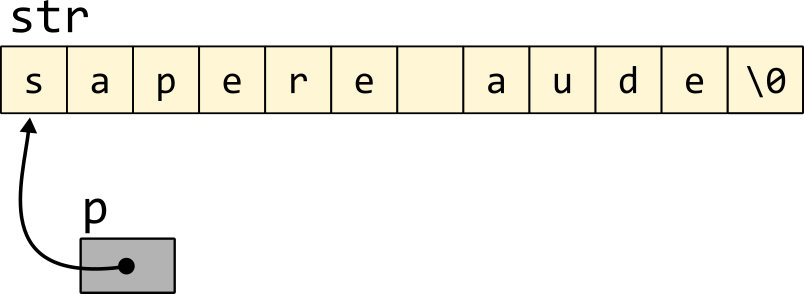
\includegraphics[scale=0.8]{../images/pointer_schemes/pointer_to_char_array.png}
\end{center}
\end{multicols}

\begin{enumerate}
\item Переведите в верхний регистр первую букву строки, используя только указатель \texttt{p}. Нужно использовать только указатель \texttt{p}, саму строку \texttt{str} использовать нельзя. Решение -- 1 строка.
\item Переведите в верхний регистр первую букву второго слова строки, используя только указатель \texttt{p}. Нужно использовать только указатель \texttt{p}, саму строку \texttt{str} использовать нельзя. Решение -- 1 строка.

\item Переведите в верхний регистр все буквы строки, используя только указатель \texttt{p}. Нужно использовать только указатель \texttt{p}, саму строку \texttt{str} использовать нельзя. Решение -- 1 цикл
\end{enumerate}


\item В следующей программе есть переменная \texttt{a} типа \texttt{int}, указатель \texttt{p} на эту переменную и указатель \texttt{q} на \texttt{p}. Удвойте значение переменной \texttt{a}, используя только указатель \texttt{q}. Нужно использовать только указатель \texttt{q}.
\begin{multicols}{2}
\begin{lstlisting}
#include <stdio.h>
int main() 
{
    int a = 1234;
    int* p = &a;
    int** q = &p;
    // Тут нужно написать 1 строку кода
    printf("%i\n", a);
}
\end{lstlisting}

\vfill \null    
\columnbreak
\vfill \null 


\begin{center}
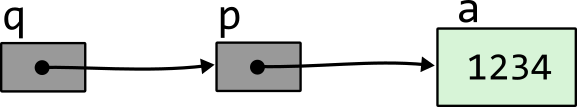
\includegraphics[scale=1]{../images/pointer_schemes/pointer_to_pointer_to_int.png}
\end{center}
\end{multicols}
\item В следующей программе была создана структура \texttt{a} типа \texttt{Date} и указатель на эту структуру. Добавьте \texttt{1} к значению поля \texttt{year}, используя только указатель \texttt{p}.
\begin{multicols}{2}
\begin{lstlisting}
#include <stdio.h>
struct date 
{
    int day, month, year;
};
typedef struct date Date;
int main() 
{
    Date a = {15, 5, 1970};
    Date* p = &a;
    // Тут нужно написать 1 строку кода
    printf("%d %d %d\n", 
           a.day, a.month, a.year);
}
\end{lstlisting}

\vfill \null    
\columnbreak
\vfill \null 

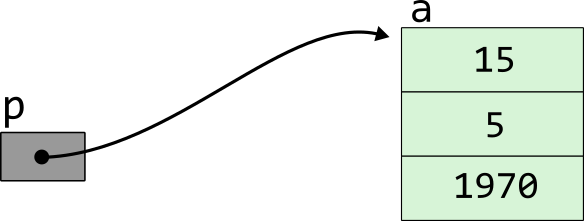
\includegraphics[scale=1]{../images/pointer_schemes/pointer_to_struct_date.png}
\end{multicols}

\newpage


\item В следующей программе была создана структура \texttt{a} типа \texttt{Movie} и указатель на неё.
\begin{multicols}{2}
\begin{lstlisting}
#include <stdio.h>
struct date 
{
    int day, month, year;
};
typedef struct date Date;

struct movie 
{
    char title[50];
    float rating;
    Date release_date;
};
typedef struct movie Movie;
\end{lstlisting}

\vfill \null  
\columnbreak
\vfill \null  

\begin{center}
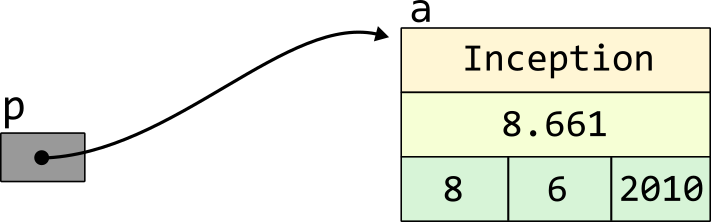
\includegraphics[scale=1]{../images/pointer_schemes/pointer_to_struct_movie.png}
\end{center}
\end{multicols}

\vspace{-10ex}
\begin{lstlisting}
int main() 
{
    Movie a = {"Inception", 8.661, {8, 6, 2010}};
    Movie* p = &a;
    // Тут нужно написать 1 строку кода
}
\end{lstlisting}
\begin{enumerate}
\item Увеличьте на \texttt{1} значение поля \texttt{rating}, используя только указатель \texttt{p}.
\item Увеличьте на \texttt{1} значение поля месяца выхода фильма, используя только указатель \texttt{p}.
\end{enumerate}





\item В следующей программе был создан массив \texttt{array} из структур типа \texttt{Movie} и указатель \texttt{p}, который указывает на второй элемент массива (\texttt{array[1]}).
\begin{lstlisting}
#include <stdio.h>
struct date 
{
    int day, month, year;
};
typedef struct date Date;

struct movie 
{
    char title[50];
    float rating;
    struct date release_date;
};
typedef struct movie Movie;

int main() 
{
    Movie array[3] = {{"Inception", 8.661, {8, 6, 2010}}, 
                      {"Green Mile", 9.062, {6, 12, 1999}}, 
                      {"Leon", 8.679, {14, 9, 1994}}};
    Movie* p = &array[1];
}
\end{lstlisting}

\vspace{-59ex}
\begin{center}
\quad\quad\quad\quad\quad\quad\quad\quad\quad\quad\quad\quad\quad\quad\quad\quad\quad\quad\quad\quad\quad\quad\quad
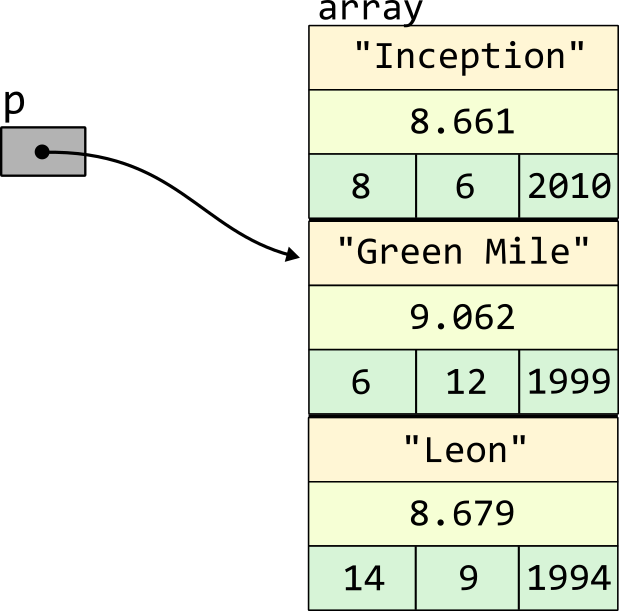
\includegraphics[scale=1]{../images/pointer_schemes/pointer_to_array_of_struct_movie.png}
\end{center}

\begin{enumerate}
\item Увеличьте на \texttt{1} значение рейтинга фильма \texttt{Inception}, используя только указатель \texttt{p}. При этом менять \texttt{p} нельзя, он  должен указывать на \texttt{array[1]}.
\item Удвойте значение года выхода фильма \texttt{Leon}, используя только указатель \texttt{p}. При этом менять \texttt{p} нельзя, он  должен указывать на \texttt{array[1]}.
\end{enumerate}

\end{enumerate}

\newpage
\subsection{Передача в функцию по указателю}
\subsection*{Передача в функцию по значению}
\begin{multicols}{2}
\begin{lstlisting}
#include <stdio.h>
struct movie 
{
    char title[50];
    float rating;
    struct date release_date;
};
typedef struct movie Movie;

void change_rating(Movie m) 
{
    m.rating += 1;
}
int main() 
{
    Movie a = {"Inception", 8.661, 
                {8, 6, 2010}};
    change_rating(a);
}
\end{lstlisting}
\columnbreak
\begin{center}
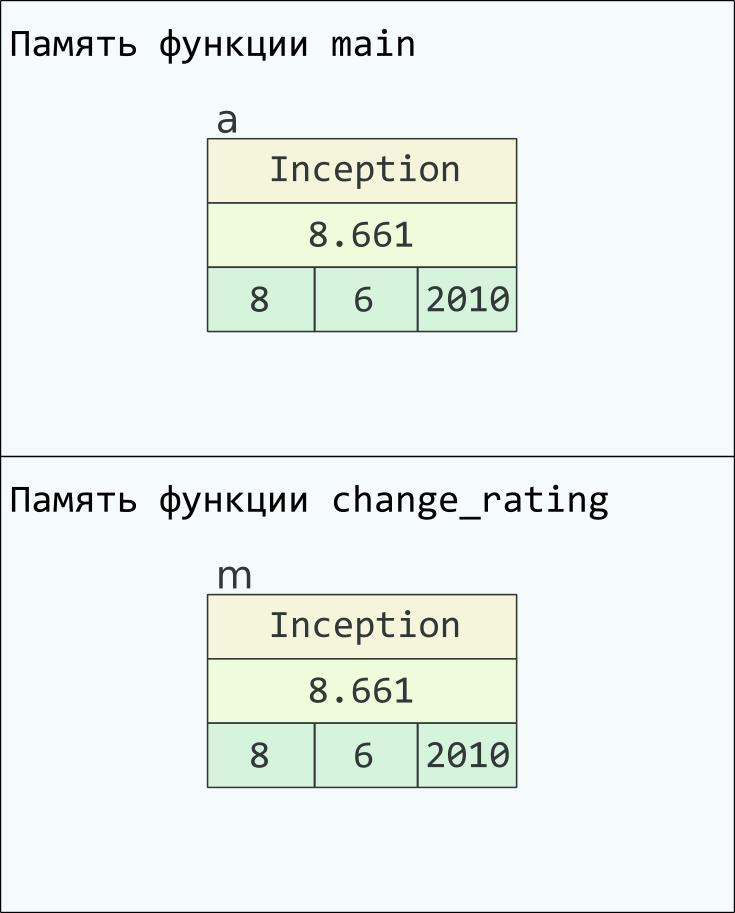
\includegraphics[scale=0.8]{../images/pointer_schemes/function_by_value.png}
\end{center}
\end{multicols}
Всё, что передаётся в функцию, копируется (кроме массивов). Поэтому функция \texttt{change\_rating} будет менять
поле \texttt{rating} у копии структуры \texttt{a}, а изначальная структура не изменится.

\subsection*{Передача в функцию по указателю:}
\begin{multicols}{2}
\begin{lstlisting}
#include <stdio.h>
struct movie 
{
    char title[50];
    float rating;
    struct date release_date;
};
typedef struct movie Movie;

void change_rating(Movie* pm) 
{
    pm->rating += 1;
}
int main() 
{
    Movie a = {"Inception", 8.661, 
              {8, 6, 2010}};
    Movie* p = &a;
    change_rating(&a);
}
\end{lstlisting}
\columnbreak
\begin{center}
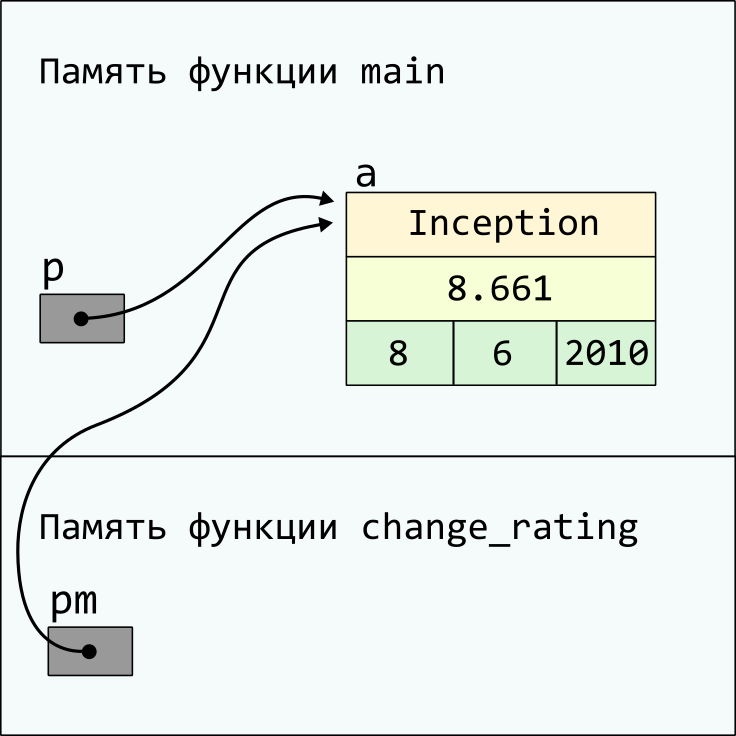
\includegraphics[scale=0.8]{../images/pointer_schemes/function_by_pointer.png}
\end{center}
\end{multicols}
Теперь в функцию копируется указатель, который содержит
адрес стурктуры \texttt{a}. Используя этот указатель, мы можем изменить изначальную структуру. Более того, так как указатель занимает меньше памяти, его копирования в функцию происходит быстрее, чем копирование всей структуры.

\subsection*{Подзадачи:}
\begin{enumerate}

\item Напишите функцию \texttt{void increase\_rating(Movie* p)}, которая будет принимать указатель типа \texttt{Movie*} и увеличивать рейтинг фильма, на которой указывает \texttt{p}, на 1.

\item Напишите функцию \texttt{void change\_year\_of\_movies(Movie* p, int size)}, которая принимает на вход указатель на первый элемент массива структур типа \texttt{Movie} и размер этого массива. Функция должна увеличивать год выхода всех фильмов на \texttt{1}. Протестируйте функции, вызвав их из функции \texttt{main} с помощью следующего кода:

\begin{lstlisting}
#include <stdio.h>
struct date 
{
    int day, month, year;
};
typedef struct date Date;
struct movie 
{
    char title[50];
    float rating;
    struct date release_date;
};
typedef struct movie Movie;

void print_date(const Date* pd) 
{
    printf("%02d.%02d.%04d", pd->day, pd->month, pd->year);
}
void print_movie(const Movie* pm) 
{
    printf("Title: %s\nRating: %.2f\nDate: ", pm->title, pm->rating);
    print_date(&pm->release_date);
    printf("\n");
}
// Тут вам нужно написать функции increase_rating и change_year_of_movies

int main() 
{
    Movie a[3] = {{"Inception", 8.661, {8, 6, 2010}}, 
                  {"Green Mile", 9.062, {6, 12, 1999}}, 
                  {"Leon", 8.679, {14, 9, 1994}}};
    increase_rating()
    change_year_of_movies(a, 3);
    for (int i = 0; i < 3; ++i)
        print_movie(&a[i]);
}
\end{lstlisting}

\end{enumerate}

\newpage
\subsection{Структура Актёр}
Напишем структуру \texttt{Actor}, в которой будем хранить информацию об одном актёре:
\begin{lstlisting}
struct actor 
{
    char name[32];
    char surname[32];
    int gender;
    int height;
    Date birth_date;
    Address birth_address;
};
typedef struct actor Actor;
\end{lstlisting}

Поля структуры \texttt{Actor}:
\begin{itemize}
\item \texttt{name} -- имя актёра
\item \texttt{surname} -- фамилия
\item \texttt{gender} -- пол (\texttt{0}, если это мужчина; \texttt{1}, если это женщина)
\item \texttt{height} -- рост в сантиметрах
\item \texttt{birth\_date} -- дата рождения (структура, содержащая 3 числа)
\item \texttt{birth\_address} -- место рождения (структура, содержащая 3 строки: страна, регион и город)
\end{itemize}


\subsection*{Файл \texttt{actors.csv}:}
В файле \texttt{actors.csv} содержится информация о 2000 актёрах (все данные сгенерированы случайным образом). Файл имеет следующий вид:
\begin{verbatim}
2000
Abel,Garifullin,0,189,16/2/1992,Russia,Rostovskaya Oblast,Rostov-na-Donu
Viktor,Shchyotkin,0,162,28/6/1992,Russia,Samarskaya Oblast,Samara
Sophia,Sigayeva,1,148,30/1/1963,Russia,Kurskaya Oblast,Zheleznogorsk
Vlada,Solodnikova,1,163,16/7/2004,Russia,Sverdlovskaya Oblast,Polevskoy
... (всего 2000 записей) ...
\end{verbatim}
Файлы формата \texttt{.csv} можно открывать как обычным текстовым редактором, так и с помощью программы для работы с табличными данными (например, Excel). 

\subsubsection*{Подзадачи:}
В файле \texttt{actors.c} содержится начальный код, нужный для решения следующих задач.
\begin{enumerate}
\item \textbf{Заданный рост:} Напишите функцию, которая будет принимать на вход массив из актёров и заданный рост и будет печатать всех актёров, которые имеют этот рост. Прототип функции:\\
\texttt{void print\_all\_actors\_by\_height(const Actor* actors, int number\_of\_actors, int height)}
\item \textbf{Заданный город:} Напишите функцию, которая будет принимать на вход массив из актёров и название города и будет печатать всех актёров, которые родились в этом городе. Прототип функции:\\
\texttt{void print\_all\_actors\_by\_city(const Actor* actors, int number\_of\_actors, char city[])}\\
Для сравнения строк используйте функцию \texttt{strcmp} из библиотеки \texttt{string.h}.
\end{enumerate}


\newpage
\subsection{Структуры Фильм  и структура База Фильмов}
Напишем структуру \texttt{Movie}, в которой будет хранить всю информацию об одном фильме:
\begin{lstlisting}
struct movie 
{
    char title[50];
    Date release_date;
    double rating;
    int crew_size;
    int crew[20];
};
typedef struct movie Movie;
\end{lstlisting}
\subsubsection*{Поля структуры \texttt{Movie}:}
\begin{itemize}
\item \texttt{title} -- название фильма (не более 49 символов)
\item \texttt{release\_date} -- дата выхода фильма (структура \texttt{Date})
\item \texttt{rating} -- рейтинг фильма
\item \texttt{crew\_size} -- количество актёров, задействованных в этом фильме
\item \texttt{crew} -- индексы актёров в массиве \texttt{actors} структуры \texttt{MovieDatabase}. Нумерация начинается с \texttt{0}.
\end{itemize}

Также напишем структуру \texttt{MovieDatabase} в котором будем хранить информацию о базе данных фильмов. Она будет содержать информацию о множестве актёров и фильмов. При этом массив актёров и фильмов будут иметь фиксированный размер (потому что создавать массив произвольной длины мы пока не умеем -- научимся только на следующих семинарах).
\begin{lstlisting}
struct movie_database 
{
    int number_of_actors;
    Actor actors[5000];
    int number_of_movies;
    Movie movies[5000]; 
};
typedef struct movie_database MovieDatabase;
\end{lstlisting}

\subsubsection*{Поля структуры \texttt{MovieDatabase}:}
\begin{itemize}
\item \texttt{number\_of\_actors} -- количество актёров в базе данных (не более 5000)
\item \texttt{actors} -- массив из всех актёров
\item \texttt{number\_of\_movies} -- количество фильмов в базе данных (не более 5000)
\item \texttt{movies} -- массив из всех фильмов
\end{itemize}

Это, конечно, не самый лучший способ для работы с базой данных. Гораздо лучший способ -- использование систем управления базами данных и библиотек для работы с ними, но это выходит за рамки данного курса.

\subsubsection*{Файл \texttt{movies.csv}:}
В файле \texttt{movies.csv} содержится информация о 4000 фильмах (все данные сгенерированы случайным образом). Файл имеет следующий вид:
\begin{verbatim}
4000
Dingy King,14/1/1980,7.402,2,1485 1932
Admire The Home,28/9/1973,6.504,9,673 814 1087 926 38 1378 629 1080 71
Egocentric Airport,24/7/1983,4.773,11,116 1747 958 40 892 1403 1752 338 62 590 1861
Stuff And The Heat,27/12/1995,6.013,9,1574 53 692 210 908 463 705 232 1582
... всего 4000 записей ...
\end{verbatim}

\newpage
\subsubsection*{Передача структур в функции:}
Видно, что структура \texttt{MovieDatabase} имеет очень большой размер (\texttt{1680016} байт!). Передавать такой размер в функцию по значению вот так:
\begin{lstlisting}
void some_function(MovieDatabase md, ...)
\end{lstlisting} 
очень плохая идея. Ведь при передаче в функцию всё копируется и это означает, что при каждом вызове такой функции будет происходить копирование всей базы фильмов. Решение -- использование указателей:
\begin{lstlisting}
void some_function(MovieDatabase* pmd, ...)
\end{lstlisting}
Теперь при вызове функции копироваться будет только указатель (всего 8 байт) и, зная адрес структуры, мы сможем получать доступ ко всем её элементам как и раньше. Однако, передавая так структуру в неизвестную нам функцию (например, функцию, которую написал другой программист), мы не можем гарантировать, что она не изменится внутри. Это ведёт к усложнению программирования, так как теперь нам нужно следить за всеми структурами при их передаче в функции (а это не так просто, ведь функции могут вызывать другие функции, а исходный код многих библиотечных функций может быть вообще неизвестен). Решение этой проблемы -- использование модификатора (\texttt{const}):
\begin{lstlisting}
void some_function(const MovieDatabase* pmd, ...)
\end{lstlisting}
Теперь структуру на которую указывает \texttt{pmd} нельзя поменять внутри функции.

\begin{center}
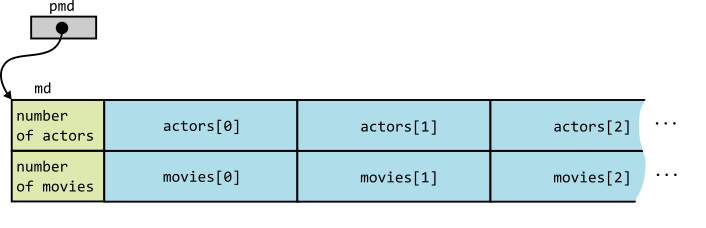
\includegraphics[scale=0.8]{../images/movie_database_structure.png}
\end{center}

\subsubsection*{Подзадачи:}
В файле \texttt{movies.c} содержится начальный код, нужный для решения следующих задач.
\begin{enumerate}
\item \textbf{Лучший фильм x4:} Напишите 4 функции, каждая из которых будет находить лучший фильм, при этом возвращая  результат разными путями. 
\begin{itemize}
\item \texttt{Movie find\_best\_movie\_value(const MovieDatabase* pmd)}\\
Возвращает структуру
\item \texttt{int find\_best\_movie\_index(const MovieDatabase* pmd)} \\
Возвращает номер фильма -- индекс в массиве \texttt{pmd->movies}
\item \texttt{const Movie* find\_best\_movie\_pointer(const MovieDatabase* pmd)}\\
Возвращает указатель на нужную структуру
\item \texttt{void find\_best\_movie\_argument(const MovieDatabase* pmd, Movie* p\_best\_movie)}\\
Записывает лучший фильм в структуру по адресу \texttt{p\_best\_movie}.
\end{itemize}
Вызовите все эти функции из \texttt{main}.
\item \textbf{Фильмография:} На вход подаётся 2 строки: имя и фамилия актёра. Напечатайте все фильмы с его участием.
\item \textbf{Лучший актёр:} Напишите функцию, которая будет находить лучшего актёра (актёра с самым большим средним рейтингом фильмов с его/её участием). Вызовите эту функцию из \texttt{main} и напечатайте этого актёра на экран.
\item \textbf{Фильмы года:} Напечатайте на экран все фильмы, вышедшие в определённый год. все фильмы должны быть отсортированы по рейтингу (от лучшего к худшему).
\end{enumerate}

\end{document}